\chapter{Figuras, tabelas, quadros, equações e algoritmos}\label{chap:elementos}
Este capítulo retoma os exemplos práticos da versão 1.4. Figuras, tabelas, equações e algoritmos recebem numeração automática e podem ser citados com \verb|\label| e \verb|\ref|. O conteúdo foi reorganizado para facilitar a substituição pelos elementos da pesquisa.

\section{Figuras}
A Figura~\ref{fig:uesc} apresenta o brasão institucional utilizado como exemplo. A identificação da fonte deve acompanhar a figura.
\begin{figure}[htbp]\centering

\includegraphics[width=0.27\textwidth]{figuras/brasao-uesc-oficial.png}
\caption{Brasão da Universidade Estadual de Santa Cruz.}\label{fig:uesc}
\fonte{Material institucional do modelo original.}
\end{figure}

\subsection{Figuras lado a lado}
A Figura~\ref{fig:comparacao} ilustra o uso de subfiguras, preservando as imagens exemplificativas do projeto 1.4. As legendas históricas originais são mantidas apenas como demonstração de composição visual, sem afirmação de data ou proveniência das fotografias.
\begin{figure}[htbp]\centering
\begin{subfigure}[b]{0.43\textwidth}\centering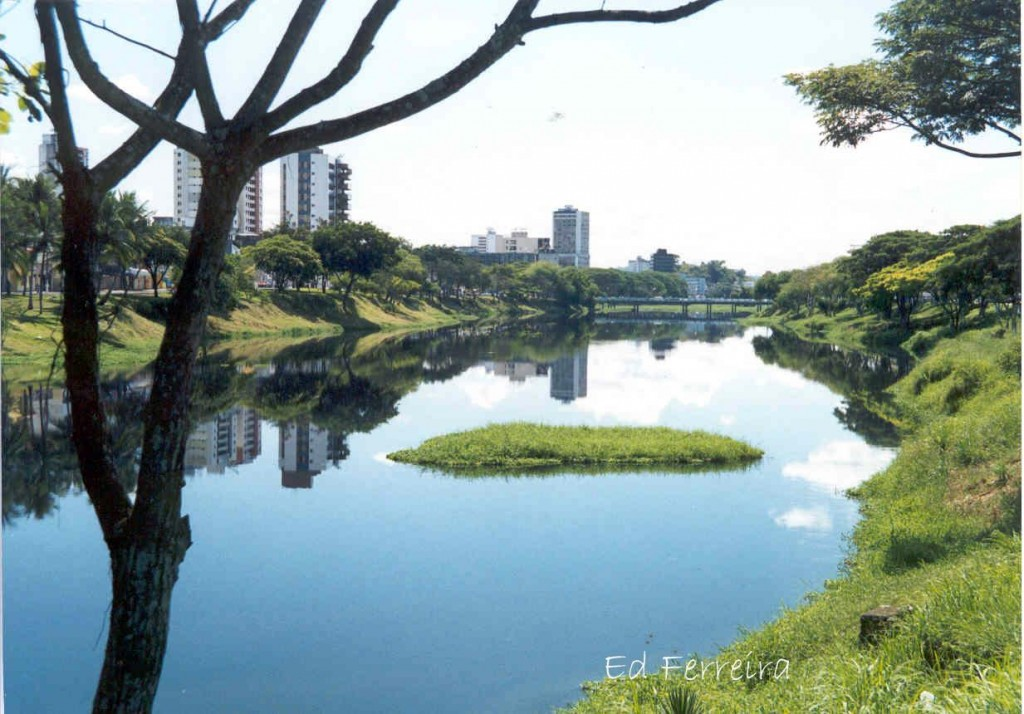
\includegraphics[width=\linewidth]{figuras/rc-adezanos.jpg}\caption{Imagem A.}\end{subfigure}\hfill
\begin{subfigure}[b]{0.43\textwidth}\centering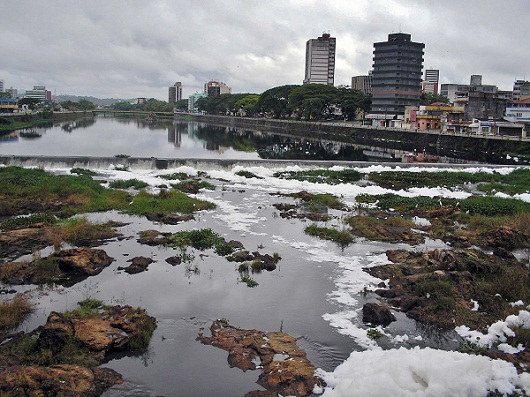
\includegraphics[width=\linewidth]{figuras/rc-atualmente.jpg}\caption{Imagem B.}\end{subfigure}
\caption{Exemplo de comparação de imagens lado a lado.}\label{fig:comparacao}
\fonte{Imagens demonstrativas preservadas da versão 1.4; proveniência a conferir.}
\end{figure}

\section{Quadros e tabelas}
O Quadro~\ref{qua:comparacao} organiza informações qualitativas, enquanto a Tabela~\ref{tab:resultados} apresenta dados numéricos ilustrativos. Não trate os valores de exemplo como resultados científicos.
\begin{quadro}[htbp]\centering\caption{Comparação qualitativa de abordagens.}\label{qua:comparacao}
\begin{tabularx}{\textwidth}{|X|X|}\hline
\textbf{Abordagem A} & \textbf{Abordagem B}\\\hline
Implementação de referência. & Implementação alternativa.\\\hline
Ênfase na precisão. & Ênfase no custo computacional.\\\hline
\end{tabularx}\\[2pt]\fonte{Elaboração própria; exemplo didático.}
\end{quadro}

\begin{table}[htbp]\centering\caption{Resultados numéricos demonstrativos.}\label{tab:resultados}
\begin{tabular}{lrrr}\toprule Caso & Erro & Tempo (s) & Iterações\\\midrule
A & 0,012 & 1,80 & 120\\
B & 0,008 & 2,40 & 180\\
C & 0,005 & 3,10 & 240\\\bottomrule
\end{tabular}\\[2pt]\fonte{Valores fictícios exclusivamente para exemplificar a formatação.}
\end{table}

\section{Equações e sistemas}
A transformada de Laplace da função $x(t)$ é apresentada na Equação~\ref{eq:laplace}:
\begin{equation}\label{eq:laplace}X(s)=\int_0^\infty x(t)e^{-st}\,\mathrm{d}t.\end{equation}
A transformada discreta de Fourier bidimensional pode ser escrita como
\begin{equation}\label{eq:dft}F(u,v)=\sum_{m=0}^{M-1}\sum_{n=0}^{N-1}f(m,n)\exp\!\left[-2\pi i\left(\frac{um}{M}+\frac{vn}{N}\right)\right].\end{equation}
Um sistema linear e uma matriz de exemplo são representados por
\begin{equation}\label{eq:sistema}A\mathbf{x}=\mathbf{b},\qquad A=\begin{bmatrix}2&-1\\-1&2\end{bmatrix},\quad \mathbf{b}=\begin{bmatrix}1\\0\end{bmatrix}.\end{equation}

\section{Algoritmos}
O Algoritmo~\ref{alg:iterativo} exemplifica a escrita de pseudocódigo com entrada, saída, condição e laço. A lógica é ilustrativa e não substitui um método de pesquisa validado.
\begin{algorithm}[htbp]
\caption{Iteração com critério de parada}\label{alg:iterativo}
\KwIn{Aproximação inicial $x_0$, tolerância $\varepsilon$, limite $N$}
\KwOut{Aproximação $x$}
$x\leftarrow x_0$; $k\leftarrow 0$\;
\While{$k<N$}{
 calcular $x_{\mathrm{novo}}$ a partir de $x$\;
 \If{$\lVert x_{\mathrm{novo}}-x\rVert<\varepsilon$}{\Return $x_{\mathrm{novo}}$\;}
 $x\leftarrow x_{\mathrm{novo}}$\; $k\leftarrow k+1$\;
}
\Return $x$\;
\end{algorithm}

\subsection{Comandos úteis para algoritmos}
O pacote \texttt{algorithm2e} oferece estruturas como \verb|\While|, \verb|\For|, \verb|\If| e \verb|\KwIn|. Os ambientes devem ser acompanhados de legenda e referência cruzada quando citados no texto.
